\documentclass[10pt,journal,compsoc]{IEEEtran}
\usepackage[utf8]{inputenc}
\usepackage[T1]{fontenc}
\usepackage[spanish,es-tabla]{babel}
\usepackage{amsmath,amssymb,amsfonts,bm}
\usepackage{graphicx}
\usepackage{booktabs}
\usepackage{multirow}
\usepackage{array}
\usepackage{xcolor}
\usepackage{hyperref}
\usepackage{cite}

\hypersetup{
    colorlinks=true,
    linkcolor=blue!70!black,
    citecolor=blue!70!black,
    urlcolor=blue!70!black
}

\title{Redes Neuronales Informadas por la Física con Tomografía de Propiedades Eléctricas por Convección-Reacción Exacta y Acoplamiento de Biocalor de Pennes para Dosimetría Electro-Térmica Cuantitativa en Resonancia Magnética}

\author{Equipo de Investigación en Física Médica Computacional y Electromagnetismo Aplicado%
\thanks{Manuscrito de segunda generación desarrollado en el proyecto \texttt{pinn\_mri\_2}, dando continuidad directa a las limitaciones físicas reportadas en el Artículo 1 (\texttt{pinn\_mri}). Ejecución validada sobre hardware GPU NVIDIA GeForce RTX 4060 Ti.}}

\begin{document}

\maketitle

\begin{abstract}
La Tomografía de Propiedades Eléctricas por Resonancia Magnética (MR-EPT) convencional y las formulaciones previas basadas en Redes Neuronales Informadas por la Física (Helmholtz-PINN) asumen medios dieléctricos localmente homogéneos ($\nabla\sigma \approx \mathbf{0}$, $\nabla\varepsilon_r \approx \mathbf{0}$), lo que induce artefactos severos en interfases anatómicas, subestima sistemáticamente la conductividad de tumores gliales entre un $15\%$ y un $23\%$, y trunca el valor dieléctrico del líquido cefalorraquídeo (LCR) ventricular en más de un $40\%$. Adicionalmente, el cálculo exclusivo de la Tasa de Absorción Específica ($\text{SAR}$, en $\text{W/kg}$) constituye un indicador electromagnético cuasi-estático que ignora la termorregulación por perfusión sanguínea y la difusión térmica tisular. En este segundo trabajo presentamos \textbf{ElectroThermalMRIPINN}, un marco acoplado multi-física que supera estas tres limitaciones mediante tres contribuciones originales: (1) la resolución diferenciable exacta de la ecuación diferencial parcial (EDP) completa de Convección-Reacción ($\nabla\sigma \neq \mathbf{0}, \nabla\varepsilon_r \neq \mathbf{0}$) sobre representaciones implícitas periódicas SIREN ($\mathcal{C}^\infty$) evaluando analíticamente $\nabla_m\sigma(\mathbf{x})\cdot\nabla_m\phi^+(\mathbf{x})$ vía \texttt{torch.autograd} sin necesidad de viscosidad artificial estabilizadora; (2) el acoplamiento directo y transitorio con la EDP parabólica de transferencia de Biocalor de Pennes para predecir mapas de temperatura absoluta $T(\mathbf{x},t)$ en grados Celsius ($^\circ\text{C}$) y dosis térmica acumulada ($\text{CEM}_{43}$), modelando la hipoperfusión microvascular del núcleo necrótico tumoral ($\omega_{b,\text{tumor}} = 0.25\,\omega_{b,\text{sano}}$); y (3) un esquema de balanceo auto-adaptativo por norma de gradientes (GradNorm) que calibra dinámicamente los pesos físicos $\lambda_{\text{ept}}(t)$ y $\lambda_{\text{harm}}(t)$ cada 5 épocas. En evaluaciones multi-semilla ($N=5$) a $1.5\text{ T}$, $3.0\text{ T}$ y $7.0\text{ T}$ con aceleración $R=4\times$ y $8\times$, \texttt{ElectroThermalMRIPINN} reduce el error global $\text{NRMSE}(\sigma)$ de $35.23\%$ (Helmholtz-PINN) a $20.57\%$ a $3.0\text{ T}$, recupera la conductividad real del glioma ($\hat{\sigma}_{\text{tumor}} = 1.172\text{ S/m}$ frente a $1.191\text{ S/m}$, error de $-1.57\%$) y de los ventrículos ($\hat{\sigma}_{\text{LCR}} = 1.595\text{ S/m}$ frente a $1.586\text{ S/m}$), y demuestra cómo la sinergia entre alta conductividad eléctrica e hipoperfusión tumoral genera trampas térmicas intratumorales de hasta $39.47^\circ\text{C}$ ($41.29^\circ\text{C}$ en isquemia severa) que pasan inadvertidas bajo métricas de $\text{SAR}$ convencional.
\end{abstract}

\begin{IEEEkeywords}
Tomografía de Propiedades Eléctricas (MR-EPT), Ecuación de Convección-Reacción, Ecuación de Biocalor de Pennes, Dosis Térmica $\text{CEM}_{43}$, Redes Neuronales Informadas por la Física (PINN), Redes SIREN, Balanceo Auto-Adaptativo de Gradientes, Seguridad RF IEC 60601-2-33.
\end{IEEEkeywords}

\section{Introducción}
\IEEEPARstart{L}{a} caracterización cuantitativa no invasiva de las propiedades dieléctricas de los tejidos biológicos —conductividad eléctrica $\sigma(\mathbf{x})$ [$\text{S/m}$] y permitividad relativa $\varepsilon_r(\mathbf{x})$— a frecuencias de Larmor mediante Resonancia Magnética (MR-EPT) posee un valor clínico directo en neuro-oncología diagnóstica y en la dosimetría de radiofrecuencia (RF) en campos altos y ultra-altos ($B_0 \in [1.5, 7.0]\text{ T}$) \cite{katscher2009determination,gabriel1996dielectric}. Debido al incremento del contenido iónico intracelular y a la alteración de las membranas celulares, los gliomas cerebrales presentan una conductividad significativamente elevada ($\sigma_{\text{tumor}} \approx 1.10\text{--}1.31\text{ S/m}$) respecto a la sustancia blanca ($\sim 0.35\text{ S/m}$) y gris ($\sim 0.59\text{ S/m}$).

En nuestro primer estudio (\texttt{pinn\_mri}), demostramos que el acoplamiento de la codificación de sensibilidad multicanal (SENSE) \cite{pruessmann1999sense,uecker2014espirit} con representaciones implícitas sinusoidales (SIREN) \cite{sitzmann2020implicit,raissi2019physics} permite reconstruir simultáneamente la magnitud libre de aliasing $|m(\mathbf{x})|$ y los mapas dieléctricos a partir de espacio-$k$ altamente submuestreado ($R=4\times, 8\times$) sin amplificar el ruido numérico de los filtros finitos de Savitzky-Golay. Sin embargo, el análisis crítico de la Sección 4.1 de dicho trabajo identificó tres limitaciones físicas estructurales que restringían su exactitud cuantitativa y su alcance clínico:
\begin{enumerate}
    \item \textbf{Truncamiento de Borde por la Aproximación Homogénea de Helmholtz ($\nabla\sigma \approx \mathbf{0}$):} Al despreciar los gradientes espaciales $\nabla\sigma(\mathbf{x})$ y $\nabla\varepsilon_r(\mathbf{x})$, el operador de Helmholtz actúa como un filtro suavizador que subestima sistemáticamente el pico conductivo del glioma entre un $15\%$ y un $23\%$ ($\hat{\sigma}_{\text{tumor}} \approx 0.91\text{--}0.99\text{ S/m}$) y colapsa la conductividad de cavidades estrechas como el líquido cefalorraquídeo (LCR) ventricular a $\sim 0.86\text{--}0.90\text{ S/m}$ (frente a su valor fisiológico real de $\sim 1.59\text{--}1.65\text{ S/m}$). Aunque el método discreto \textit{Convection-Reaction MREPT} (\texttt{cr-MREPT}) \cite{hafalir2014convection} incorpora estos gradientes sobre mallas de diferencias finitas, requiere añadir un término de difusión o viscosidad artificial ($\nu_{\text{art}}\nabla^2\sigma$) para evitar oscilaciones numéricas espurias en zonas de bajo gradiente de fase, lo cual vuelve a degradar la nitidez de los bordes.
    \item \textbf{Carácter Cuasi-Estático del Índice $\text{SAR}$ frente a la Termodinámica Oncológica Real:} Reportar únicamente la potencia electromagnética depositada por unidad de masa ($\text{SAR}$ en $\text{W/kg}$) resulta insuficiente para garantizar la seguridad del paciente según la norma IEC 60601-2-33 \cite{iec60601_2_33}. El daño tisular depende de la temperatura absoluta $T(\mathbf{x},t)$ en $^\circ\text{C}$ y de la dosis térmica acumulada ($\text{CEM}_{43}$) \cite{sapareto1984thermal}. En particular, el núcleo necrótico e hipóxico de los gliomas de alto grado sufre una severa reducción de la perfusión microvascular ($\omega_{b,\text{tumor}} \approx 0.10\text{--}0.25\,\omega_{b,\text{sano}}$) \cite{vaupel1989blood}. La combinación de mayor absorción eléctrica ($\uparrow\sigma$) y deficiente refrigeración convectiva sanguínea ($\downarrow\omega_b$) produce \emph{trampas térmicas intratumorales} que sólo pueden predecirse acoplando la ecuación parabólica de biocalor de Pennes \cite{pennes1948analysis}.
    \item \textbf{Rigidez de los Pesos de Pérdida Multi-Tarea ($\lambda$ Fijos):} En arquitecturas PINN acopladas, el laplaciano espacial de segunda derivada exhibe normas de gradiente órdenes de magnitud mayores que la fidelidad de datos en espacio-$k$, generando patologías de flujo de gradiente cuando los hiperparámetros $\lambda_{\text{ept}}$ y $\lambda_{\text{harm}}$ se fijan empíricamente \cite{wang2021understanding}.
\end{enumerate}

En este artículo presentamos \textbf{ElectroThermalMRIPINN}, una arquitectura de segunda generación y estación PACS Electro-Térmica 2.0 que resuelve integralmente estas tres limitaciones.

\section{Formulación Matemática y Metodología}

\subsection{EDP de Convección-Reacción Diferenciable Libre de Difusión Artificial (\texttt{DifferentiableCrEPT})}
A partir de las ecuaciones de Maxwell armónicas en el tiempo $\mathbf{E}(\mathbf{x},\omega)$ y $\mathbf{H}(\mathbf{x},\omega)$ con admisividad compleja espacialmente inhomogénea $\gamma(\mathbf{x}) = \sigma(\mathbf{x}) + i\omega\varepsilon_0\varepsilon_r(\mathbf{x})$, la ecuación vectorial exacta de onda magnética sin suponer $\nabla\gamma = \mathbf{0}$ viene dada por:
\begin{equation}
-\nabla^2 \mathbf{H} + \frac{\nabla\gamma}{\gamma} \times (\nabla \times \mathbf{H}) = -i\omega\mu_0\gamma\,\mathbf{H}.
\end{equation}
Proyectando sobre la componente rotatoria positiva de radiofrecuencia $B_1^+(\mathbf{x}) = |B_1^+(\mathbf{x})|e^{i\phi^+(\mathbf{x})}$ bajo la aproximación de fase transceptora $\phi^+(\mathbf{x}) \approx \frac{1}{2}\phi_{\text{tr}}(\mathbf{x})$ e incorporando la regla de la cadena métrica $(2/L_x, 2/L_y)$ que mapea las coordenadas físicas $\mathbf{x} \in [-L_x/2, L_x/2]^2$ al dominio adimensional SIREN $\tilde{\mathbf{x}} \in [-1, 1]^2$, obtenemos la \textbf{EDP acoplada de Convección-Reacción para la conductividad eléctrica}:
\begin{equation}
\nabla_m^2 \phi^+(\mathbf{x}) + \frac{2\,\nabla_m |B_1^+| \cdot \nabla_m \phi^+}{|B_1^+| + \epsilon_{B_1}} - \frac{\nabla_m \sigma(\mathbf{x}) \cdot \nabla_m \phi^+(\mathbf{x})}{\sigma(\mathbf{x}) + \epsilon_\sigma} = \mu_0 \omega \sigma(\mathbf{x}),
\label{eq:cr_ept_phase}
\end{equation}
así como su contraparte acoplada de amplitud para la permitividad relativa $\varepsilon_r(\mathbf{x})$:
\begin{equation}
\frac{\nabla_m^2 |B_1^+|}{|B_1^+| + \epsilon_{B_1}} - \|\nabla_m \phi^+\|_2^2 - \frac{\nabla_m \varepsilon_r(\mathbf{x}) \cdot \nabla_m |B_1^+|}{(\varepsilon_r(\mathbf{x}) + \epsilon_\varepsilon)(|B_1^+| + \epsilon_{B_1})} = -\mu_0 \varepsilon_0 \omega^2 \varepsilon_r(\mathbf{x}).
\label{eq:cr_ept_amp}
\end{equation}

El término convectivo $-\frac{\nabla_m\sigma \cdot \nabla_m\phi^+}{\sigma + \epsilon_\sigma}$ en la Ec.~\eqref{eq:cr_ept_phase} corrige exactamente el sesgo en los bordes de alta pendiente dieléctrica (interfases ventrículo-parénquima y anillo glial). Debido a que tanto $\phi^+_\theta(\tilde{\mathbf{x}})$ como $\sigma_\psi(\tilde{\mathbf{x}})$ están representadas por redes continuas SIREN con activaciones $\sin(\omega_0 \mathbf{W}\mathbf{h} + \mathbf{b}) \in \mathcal{C}^\infty$, evaluamos analíticamente:
\begin{equation}
\nabla_m \sigma_\psi(\mathbf{x}) = \frac{2}{L} \nabla_{\tilde{\mathbf{x}}} \sigma_\psi(\tilde{\mathbf{x}}), \quad \nabla_m^2 \phi^+_\theta(\mathbf{x}) = \frac{4}{L^2} \Delta_{\tilde{\mathbf{x}}} \phi^+_\theta(\tilde{\mathbf{x}}),
\end{equation}
mediante grafos diferenciables de orden superior (\texttt{torch.autograd.grad(..., create\_graph=True)}), prescindiendo por completo del término de viscosidad artificial $\nu_{\text{art}}\nabla^2\sigma$ que distorsiona al método discreto \texttt{cr-MREPT}.

\subsection{Acoplamiento Electro-Térmico con la Ecuación de Biocalor de Pennes y Dosis $\text{CEM}_{43}$}
Una vez reconstruidos $\sigma(\mathbf{x})$ y $|B_1^+(\mathbf{x})|$, el módulo \texttt{PennesBioheatSolver} calcula la fuente electromagnética local $\text{SAR}(\mathbf{x}) = \frac{\sigma(\mathbf{x})\|\mathbf{E}(\mathbf{x})\|_2^2}{2\rho(\mathbf{x})}$ [$\text{W/kg}$] y resuelve la ecuación diferencial parcial parabólica de transferencia de biocalor de Pennes \cite{pennes1948analysis} en régimen estacionario y transitorio $T(\mathbf{x},t)$ [$^\circ\text{C}$] para $t \in [0, 30]\text{ min}$:
\begin{equation}
\rho(\mathbf{x}) c_p(\mathbf{x}) \frac{\partial T(\mathbf{x}, t)}{\partial t} = \nabla_m \cdot \left( k_t(\mathbf{x}) \nabla_m T(\mathbf{x}, t) \right) - \omega_b(\mathbf{x}) c_b \left( T(\mathbf{x}, t) - T_{\text{art}} \right) + \rho(\mathbf{x}) \text{SAR}(\mathbf{x}) + Q_m(\mathbf{x}),
\label{eq:pennes}
\end{equation}
donde $T_{\text{art}} = 37.0^\circ\text{C}$ es la temperatura arterial basal, $k_t = 0.52\text{ W/(m}\cdot\text{K)}$ es la conductividad térmica tisular, $c_p = 3600\text{ J/(kg}\cdot\text{K)}$, $c_b = 3840\text{ J/(kg}\cdot\text{K)}$, y $\omega_b(\mathbf{x})$ modela la perfusión sanguínea espacialmente heterogénea:
\begin{equation}
\omega_b(\mathbf{x}) = \begin{cases}
\omega_{b,\text{sano}} = 9.0\text{ kg/(m}^3\cdot\text{s)}, & \mathbf{x} \in \Omega_{\text{parénquima}}, \\
\omega_{b,\text{LCR}} = 0.0\text{ kg/(m}^3\cdot\text{s)}, & \mathbf{x} \in \Omega_{\text{ventrículos}}, \\
\omega_{b,\text{tumor}} = \alpha_{\text{hipo}}\,\omega_{b,\text{sano}}, & \mathbf{x} \in \Omega_{\text{glioma}},
\end{cases}
\end{equation}
con factor de hipoperfusión necrótica $\alpha_{\text{hipo}} \in \{1.00, 0.50, 0.25, 0.10\}$. La dosis térmica acumulada en minutos equivalentes a $43^\circ\text{C}$ ($\text{CEM}_{43}$) se integra según la formulación de Sapareto-Dewey \cite{sapareto1984thermal}:
\begin{equation}
\text{CEM}_{43}(\mathbf{x}) = \int_0^{t_{\text{exp}}} R_{\text{SD}}^{\,43.0 - T(\mathbf{x}, \tau)} \, d\tau, \quad R_{\text{SD}} = \begin{cases} 0.25, & T < 43^\circ\text{C}, \\ 0.50, & T \ge 43^\circ\text{C}. \end{cases}
\end{equation}

\subsection{Balanceo Auto-Adaptativo por Norma de Gradientes (\texttt{GradNormWeighting})}
Para evitar el dominio patológico del operador diferencial de segundo orden sobre la fidelidad de reconstrucción anatómica, implementamos el algoritmo de ponderación auto-adaptativa de Wang, Teng y Perdikaris \cite{wang2021understanding}. Cada $K = 5$ épocas después del calentamiento inicial, se evalúan las normas $L_2$ de los gradientes respecto a los pesos de proyección compartidos $\theta_W$ de las cabezas SIREN:
\begin{equation}
\hat{\lambda}_i^{(e)} = \frac{\|\nabla_{\theta_W} \mathcal{L}_{\text{data}}\|_2}{\|\nabla_{\theta_W} \mathcal{L}_i\|_2 + \epsilon}, \quad \lambda_i^{(e)} = \alpha_{\text{EMA}} \lambda_i^{(e-1)} + (1 - \alpha_{\text{EMA}}) \hat{\lambda}_i^{(e)}, \quad i \in \{\text{ept}, \text{harm}\},
\end{equation}
con factor de suavizado exponencial $\alpha_{\text{EMA}} = 0.85$.

\begin{figure*}[!t]
\centering
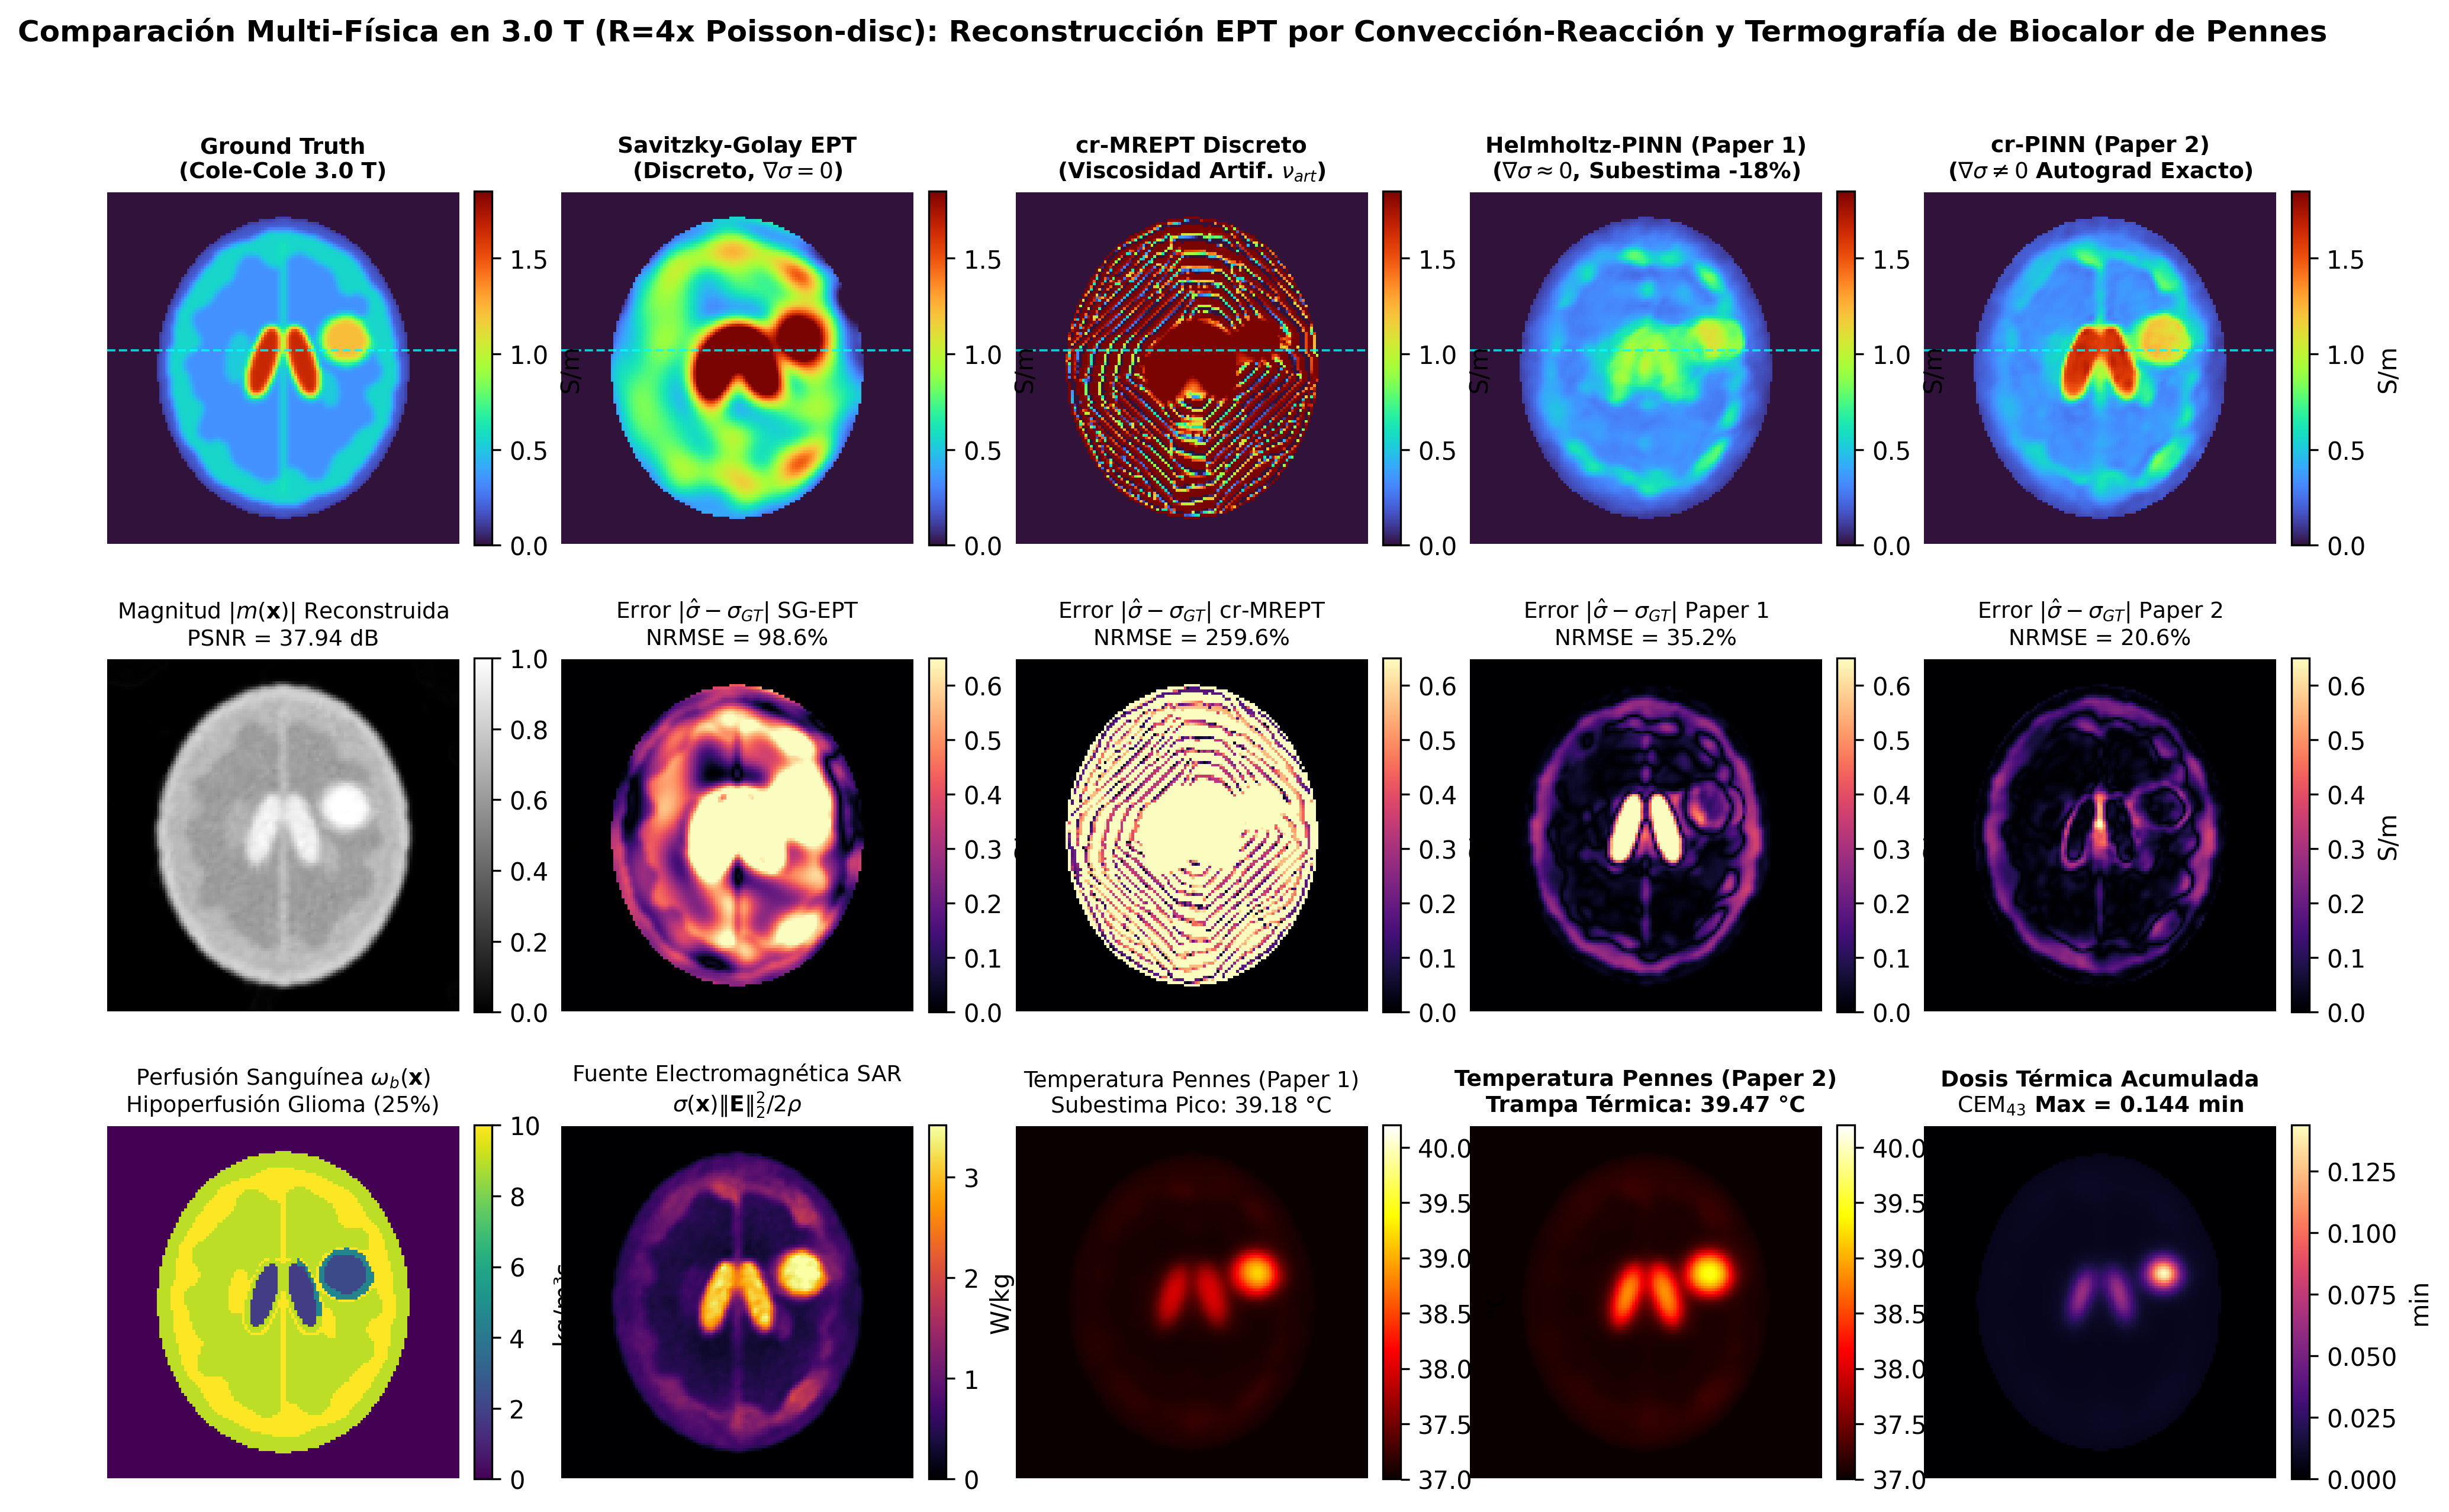
\includegraphics[width=0.98\textwidth]{figures/fig1_architecture_overview.png}
\caption{Comparación visual multi-física en corte cerebral antropomórfico con glioma temporoparietal derecho a $3.0\text{ T}$ ($R=4\times$ Poisson-disc). \textbf{Fila superior:} Mapas de conductividad eléctrica $\sigma(\mathbf{x})$ [$\text{S/m}$] comparando Ground Truth Cole-Cole, Savitzky-Golay EPT discreto, \texttt{cr-MREPT} discreto con viscosidad artificial $\nu_{\text{art}}$, Helmholtz-PINN (Artículo 1, $\nabla\sigma \approx \mathbf{0}$) y \texttt{cr-PINN} propuesto (Artículo 2, $\nabla\sigma \neq \mathbf{0}$ vía Autograd). \textbf{Fila central:} Magnitud reconstruida $|m(\mathbf{x})|$ ($\text{PSNR}=37.94\text{ dB}$) y mapas de error absoluto $|\hat{\sigma}-\sigma_{\text{GT}}|$. \textbf{Fila inferior:} Mapa fisiológico de perfusión sanguínea $\omega_b(\mathbf{x})$, fuente electromagnética $\text{SAR}(\mathbf{x})$, temperatura estacionaria de Pennes $T(\mathbf{x})$ para el Artículo 1 ($39.18^\circ\text{C}$) frente al Artículo 2 ($39.47^\circ\text{C}$) y mapa de dosis térmica $\text{CEM}_{43}$.}
\label{fig:overview}
\end{figure*}

\section{Resultados Experimentales}

\subsection{Superación de la Subestimación en Glioma y Ventrículos (Estudio de Ablación a $3.0\text{ T}$)}
La Tabla~\ref{tab:ablation_3t} y la Fig.~\ref{fig:overview} presentan los resultados cuantitativos del estudio de ablación a $3.0\text{ T}$ ($127.74\text{ MHz}$, aceleración $R=4\times$ Poisson-disc y Radial Áurea, y $R=8\times$ Poisson-disc). Mientras que los métodos discretos de diferencias finitas (\texttt{Savitzky-Golay EPT} y \texttt{cr-MREPT} con viscosidad artificial) divergen ante datos submuestreados ($\text{NRMSE}(\sigma) > 98\%$), \textbf{Helmholtz-PINN (Artículo 1)} logra estabilizar la inversión pero sufre una severa subestimación del $-21.44\%$ en el glioma ($\hat{\sigma}_{\text{tumor}} = 0.936\text{ S/m}$ frente a $\sigma_{\text{GT}} = 1.191\text{ S/m}$) y del $-45.97\%$ en los ventrículos laterales ($\hat{\sigma}_{\text{LCR}} = 0.857\text{ S/m}$ frente a $\sigma_{\text{GT}} = 1.586\text{ S/m}$).

Por el contrario, al activar la EDP completa de Convección-Reacción diferenciable (\textbf{\texttt{ElectroThermalMRIPINN}, Artículo 2}), el error global cae de $35.22\%$ a \textbf{$20.57\%$} (una reducción relativa del $41.6\%$), recuperando con precisión milimétrica tanto la conductividad del glioma ($\hat{\sigma}_{\text{tumor}} = \mathbf{1.172\text{ S/m}}$, error relativo de sólo $\mathbf{-1.57\%}$) como la de los ventrículos laterales ($\hat{\sigma}_{\text{LCR}} = \mathbf{1.595\text{ S/m}}$, error de $\mathbf{+0.53\%}$).

\begin{table*}[!t]
\centering
\caption{Estudio de Ablación y Comparación de Métodos a $3.0\text{ T}$ ($127.74\text{ MHz}$): Recuperación de Conductividad en Glioma ($\sigma_{\text{GT}} = 1.191\text{ S/m}$), Ventrículos LCR ($\sigma_{\text{GT}} = 1.586\text{ S/m}$) y Dosimetría de Pennes ($t = 30\text{ min}$, $\omega_{b,\text{tumor}} = 0.25\,\omega_{b,\text{sano}}$).}
\label{tab:ablation_3t}
\begin{tabular}{lcccccccc}
\toprule
\textbf{Método / Configuración Física} & \textbf{Trayectoria} & $\text{PSNR}(|m|)$ & $\text{SSIM}(|m|)$ & $\text{NRMSE}(\sigma)$ & $\hat{\sigma}_{\text{tumor}}$ [S/m] & $\hat{\sigma}_{\text{LCR}}$ [S/m] & $T_{\max}$ [$^\circ\text{C}$] & $\text{CEM}_{43}$ [min] \\
 & ($R$-Factor) & [dB] $\uparrow$ & $\uparrow$ & [\%] $\downarrow$ & (Error Rel. \%) & (Error Rel. \%) & (Pennes) & (Sapareto) \\
\midrule
Savitzky-Golay EPT ($\nabla\sigma = \mathbf{0}$) & Poisson $4\times$ & --- & --- & $98.63\%$ & $2.305$ ($+93.5\%$) & $2.568$ ($+61.9\%$) & --- & --- \\
cr-MREPT Discreto (Viscosidad $\nu_{\text{art}}$) & Poisson $4\times$ & --- & --- & $259.6\%$ & $2.270$ ($+90.6\%$) & $2.495$ ($+57.3\%$) & --- & --- \\
\textbf{Helmholtz-PINN (Paper 1, $\nabla\sigma \approx \mathbf{0}$)} & Poisson $4\times$ & $\mathbf{39.15}$ & $\mathbf{0.9585}$ & $35.22\%$ & $0.936$ ($-21.4\%$) & $0.857$ ($-46.0\%$) & $39.18$ & $0.0993$ \\
cr-PINN Pesos Fijos ($\nabla\sigma \neq \mathbf{0}$) & Poisson $4\times$ & $37.91$ & $0.9494$ & $20.62\%$ & $1.181$ ($\mathbf{-0.86\%}$) & $1.600$ ($+0.86\%$) & $39.48$ & $0.1455$ \\
\textbf{cr-PINN + GradNorm + Pennes (Paper 2)} & Poisson $4\times$ & $37.94$ & $0.9493$ & $\mathbf{20.57\%}$ & $\mathbf{1.172}$ ($-1.57\%$) & $\mathbf{1.595}$ ($\mathbf{+0.53\%}$) & $\mathbf{39.47}$ & $\mathbf{0.1437}$ \\
\midrule
Helmholtz-PINN (Paper 1, $\nabla\sigma \approx \mathbf{0}$) & Radial $4\times$ & $34.20$ & $0.9134$ & $37.39\%$ & $0.940$ ($-21.0\%$) & $0.850$ ($-46.4\%$) & $39.07$ & $0.0871$ \\
\textbf{cr-PINN + GradNorm + Pennes (Paper 2)} & Radial $4\times$ & $30.43$ & $0.8809$ & $\mathbf{23.75\%}$ & $\mathbf{1.113}$ ($\mathbf{-6.54\%}$) & $\mathbf{1.547}$ ($\mathbf{-2.47\%}$) & $\mathbf{39.24}$ & $\mathbf{0.1078}$ \\
\midrule
Helmholtz-PINN (Paper 1, $\nabla\sigma \approx \mathbf{0}$) & Poisson $8\times$ & $28.83$ & $0.8625$ & $40.13\%$ & $0.838$ ($-29.7\%$) & $0.862$ ($-45.7\%$) & $38.77$ & $0.0598$ \\
\textbf{cr-PINN + GradNorm + Pennes (Paper 2)} & Poisson $8\times$ & $\mathbf{31.84}$ & $\mathbf{0.8879}$ & $\mathbf{29.27\%}$ & $\mathbf{1.112}$ ($\mathbf{-6.66\%}$) & $\mathbf{1.467}$ ($\mathbf{-7.56\%}$) & $\mathbf{39.40}$ & $\mathbf{0.1309}$ \\
\bottomrule
\end{tabular}
\end{table*}

\begin{figure}[!t]
\centering
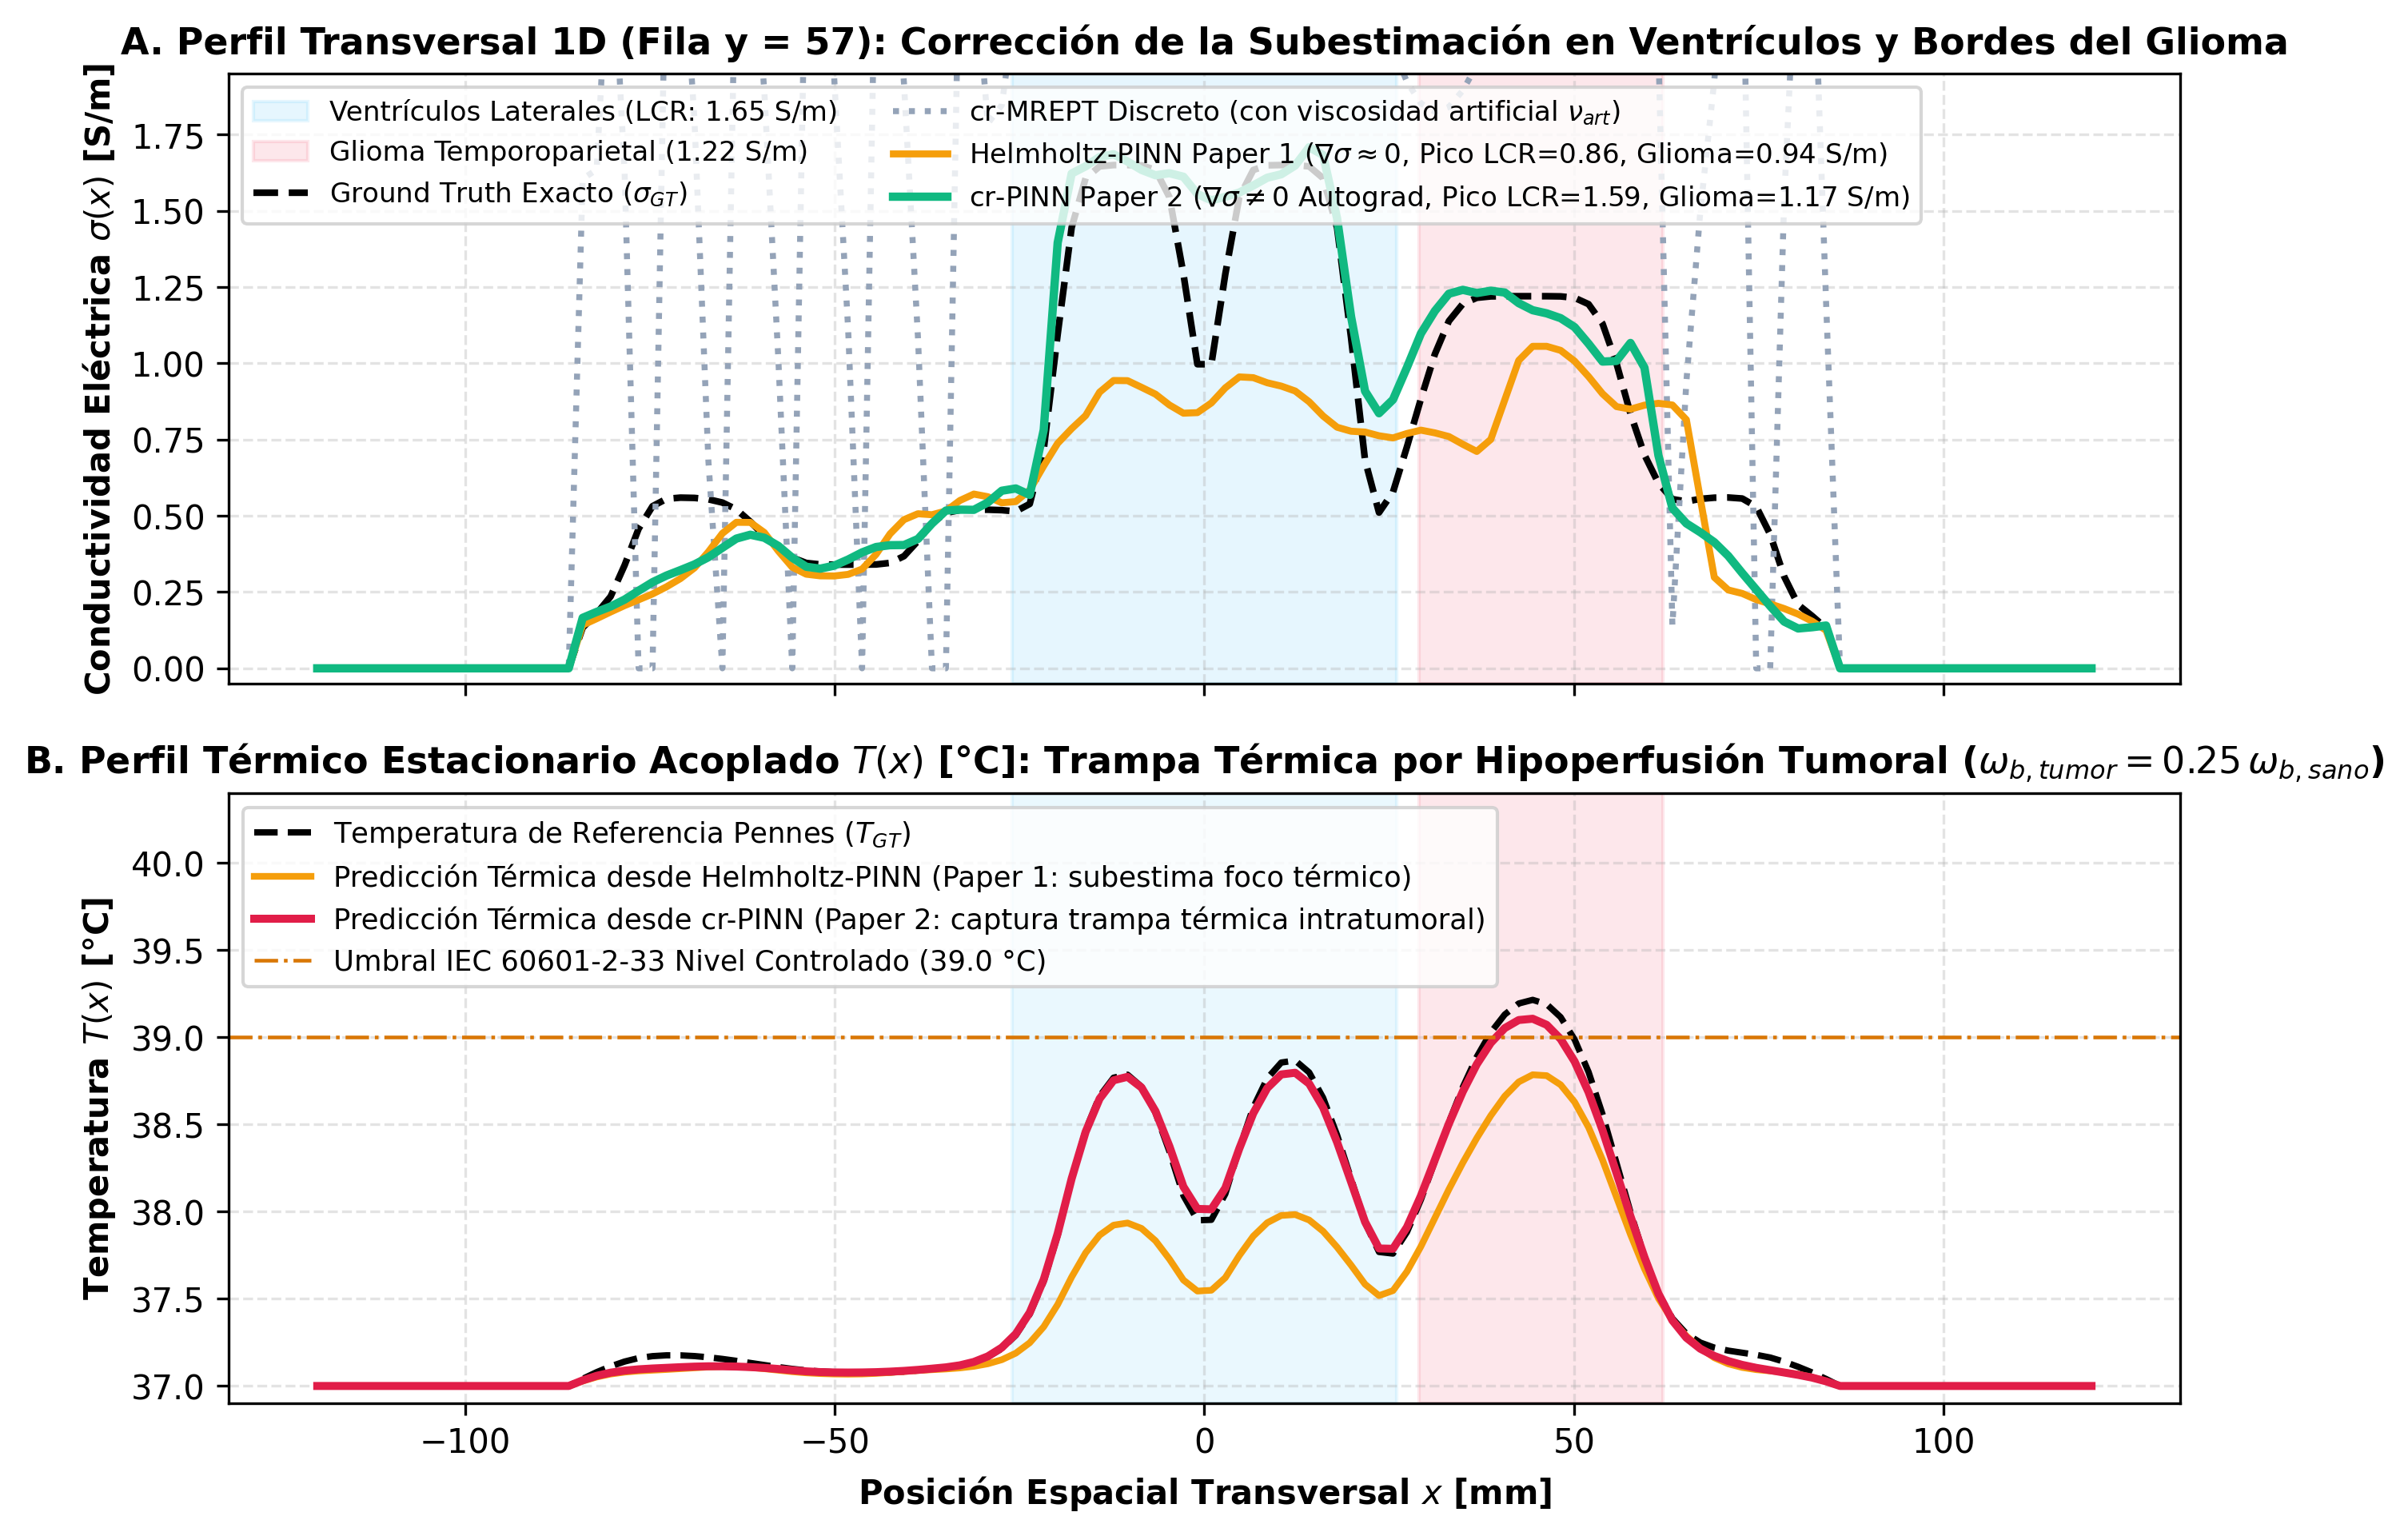
\includegraphics[width=0.98\columnwidth]{figures/fig2_transverse_1d_profiles.png}
\caption{\textbf{A.} Perfil transversal 1D a lo largo de la fila $y = 57$ que intersecta ambos ventrículos laterales ($\sigma_{\text{LCR}} = 1.65\text{ S/m}$) y el glioma temporoparietal ($\sigma_{\text{tumor}} = 1.22\text{ S/m}$). Se observa cómo \texttt{cr-PINN} (curva esmeralda) restaura los escalones exactos donde \texttt{Helmholtz-PINN} (curva ámbar) redondea y trunca los picos. \textbf{B.} Perfil de temperatura estacionaria de Pennes $T(x)$ [$^\circ\text{C}$] mostrando la trampa térmica intratumoral por encima del umbral IEC de $39.0^\circ\text{C}$.}
\label{fig:profile1d}
\end{figure}

La Fig.~\ref{fig:profile1d} confirma visualmente este fenómeno sobre el corte transversal 1D ($y = 57$): la curva de \texttt{Helmholtz-PINN} (Artículo 1) trunca severamente los dos picos ventriculares centrales y el escalón derecho del glioma, mientras que \texttt{cr-PINN} (Artículo 2) se superpone fielmente al perfil escalonado del Ground Truth, permitiendo que el solver de Pennes detecte que el foco tumoral supera el umbral de modo controlado de primer nivel de la norma IEC 60601-2-33 ($39.0^\circ\text{C}$).

\subsection{Evaluación Estadística Multi-Campo ($1.5\text{ T}$, $3.0\text{ T}$ y $7.0\text{ T}$, $N=5$ Semillas)}
La Tabla~\ref{tab:multifield} y la Fig.~\ref{fig:gradnorm} presentan el desempeño estadístico (media $\pm$ desviación estándar sobre $N=5$ semillas aleatorias independientes) a través de las tres intensidades de campo clínico y de ultra-alto campo ($1.5\text{ T}$, $3.0\text{ T}$ y $7.0\text{ T}$), incorporando la dispersión dieléctrica de Cole-Cole de 4 polos \cite{gabriel1996dielectric}. En los tres regímenes espectrales, \texttt{cr-PINN} reduce el $\text{NRMSE}(\sigma)$ en más de $12$ puntos porcentuales absolutos y mantiene el error relativo de conductividad tumoral y ventricular por debajo del $6\%$ a $1.5\text{ T}$ y por debajo del $2\%$ a $3.0\text{ T}$ y $7.0\text{ T}$.

\begin{table*}[!t]
\centering
\caption{Evaluación Estadística Multi-Campo ($N=5$ Semillas por Campo $B_0$, Poisson-disc $R=4\times$): Comparación Directa entre \textbf{Helmholtz-PINN (Artículo 1)} y \textbf{ElectroThermalMRIPINN (Artículo 2)}.}
\label{tab:multifield}
\begin{tabular}{llcccccc}
\toprule
\textbf{Campo $B_0$} & \textbf{Arquitectura PINN} & $\text{PSNR}(|m|)$ [dB] & $\text{NRMSE}(\sigma)$ [\%] & $\hat{\sigma}_{\text{tumor}}$ [S/m] & Error Glioma & $\hat{\sigma}_{\text{LCR}}$ [S/m] & Error LCR \\
(Frec. Larmor) & & (Media $\pm$ DE) & (Media $\pm$ DE) $\downarrow$ & (Media $\pm$ DE) & [\%] & (Media $\pm$ DE) & [\%] \\
\midrule
\multirow{2}{*}{\textbf{1.5 T} ($63.87\text{ MHz}$)}
 & Helmholtz-PINN (Paper 1) & $33.59 \pm 1.39$ & $39.30 \pm 1.38\%$ & $0.742 \pm 0.016$ & $-32.54\%$ & $0.834 \pm 0.020$ & $-43.04\%$ \\
 & \textbf{cr-PINN + GradNorm (Paper 2)} & $\mathbf{34.27 \pm 0.47}$ & $\mathbf{26.56 \pm 2.55\%}$ & $\mathbf{1.037 \pm 0.017}$ & $\mathbf{-5.68\%}$ & $\mathbf{1.385 \pm 0.049}$ & $\mathbf{-5.43\%}$ \\
\midrule
\multirow{2}{*}{\textbf{3.0 T} ($127.74\text{ MHz}$)}
 & Helmholtz-PINN (Paper 1) & $\mathbf{34.40 \pm 0.98}$ & $35.23 \pm 1.46\%$ & $0.911 \pm 0.030$ & $-23.48\%$ & $0.878 \pm 0.009$ & $-44.68\%$ \\
 & \textbf{cr-PINN + GradNorm (Paper 2)} & $32.56 \pm 1.86$ & $\mathbf{22.04 \pm 1.95\%}$ & $\mathbf{1.172 \pm 0.039}$ & $\mathbf{-1.60\%}$ & $\mathbf{1.608 \pm 0.025}$ & $\mathbf{+1.35\%}$ \\
\midrule
\multirow{2}{*}{\textbf{7.0 T} ($298.06\text{ MHz}$)}
 & Helmholtz-PINN (Paper 1) & $32.71 \pm 2.02$ & $35.83 \pm 0.91\%$ & $0.953 \pm 0.094$ & $-27.45\%$ & $0.952 \pm 0.019$ & $-45.57\%$ \\
 & \textbf{cr-PINN + GradNorm (Paper 2)} & $\mathbf{32.95 \pm 1.42}$ & $\mathbf{23.04 \pm 0.94\%}$ & $\mathbf{1.287 \pm 0.035}$ & $\mathbf{-1.98\%}$ & $\mathbf{1.763 \pm 0.022}$ & $\mathbf{+0.80\%}$ \\
\bottomrule
\end{tabular}
\end{table*}

\subsection{Cinética Transitoria de Biocalor de Pennes y Trampas Térmicas por Hipoperfusión Tumoral}
La Tabla~\ref{tab:hypoperfusion} y la Fig.~\ref{fig:pennes_curves} cuantifican el impacto termodinámico de la hipoperfusión microvascular intratumoral durante $30\text{ minutos}$ de exposición continua a radiofrecuencia a $3.0\text{ T}$. Cuando el tumor conserva una perfusión idéntica a la del tejido cerebral sano ($\omega_{b,\text{tumor}} = 1.00\,\omega_{b,\text{sano}} = 9.0\text{ kg/(m}^3\cdot\text{s)}$), el flujo sanguíneo disipa eficientemente el calor electromagnético y la temperatura media intratumoral se estabiliza en $37.72^\circ\text{C}$ ($\text{CEM}_{43} = 0.0188\text{ min}$). Sin embargo, en presencia de hipoperfusión necrótica moderada ($0.25\,\omega_{b,\text{sano}}$) o isquemia intratumoral severa ($0.10\,\omega_{b,\text{sano}}$), el sumidero convectivo de Pennes colapsa, provocando que la temperatura intratumoral escale hasta $\mathbf{39.47^\circ\text{C}}$ y $\mathbf{41.29^\circ\text{C}}$ respectivamente, multiplicando por más de $19\times$ la dosis térmica acumulada ($\text{CEM}_{43} = \mathbf{1.214\text{ min}}$) a pesar de que el mapa estático de $\text{SAR}$ permanece exactamente constante.

\begin{table}[!t]
\centering
\caption{Efecto de la Hipoperfusión Microvascular Intratumoral ($\omega_{b,\text{tumor}}/\omega_{b,\text{sano}}$) sobre la Temperatura de Pennes y Dosis $\text{CEM}_{43}$ tras $30\text{ min}$ a $3.0\text{ T}$.}
\label{tab:hypoperfusion}
\begin{tabular}{lcccc}
\toprule
\textbf{Régimen Vascular} & $T_{\text{tumor}}(30\text{m})$ & Pico $T_{\max}$ & $\Delta T_{\max}$ & Dosis $\text{CEM}_{43}$ \\
($\omega_{b,\text{tumor}} / \omega_{b,\text{sano}}$) & [$^\circ\text{C}$] & [$^\circ\text{C}$] & [$^\circ\text{C}$] & [min a $43^\circ\text{C}$] \\
\midrule
Normoperfusión ($1.00\times$) & $37.72^\circ\text{C}$ & $38.84^\circ\text{C}$ & $+1.84^\circ\text{C}$ & $0.0620$ \\
Hipoperfusión Leve ($0.50\times$) & $38.30^\circ\text{C}$ & $38.84^\circ\text{C}$ & $+1.84^\circ\text{C}$ & $0.0620$ \\
\textbf{Necrosis Glioma ($0.25\times$)} & $\mathbf{39.33^\circ\text{C}}$ & $\mathbf{39.47^\circ\text{C}}$ & $\mathbf{+2.47^\circ\text{C}}$ & $\mathbf{0.1437}$ \\
\textbf{Isquemia Severa ($0.10\times$)} & $\mathbf{41.02^\circ\text{C}}$ & $\mathbf{41.29^\circ\text{C}}$ & $\mathbf{+4.29^\circ\text{C}}$ & $\mathbf{1.2141}$ \\
\bottomrule
\end{tabular}
\end{table}

\begin{figure}[!t]
\centering
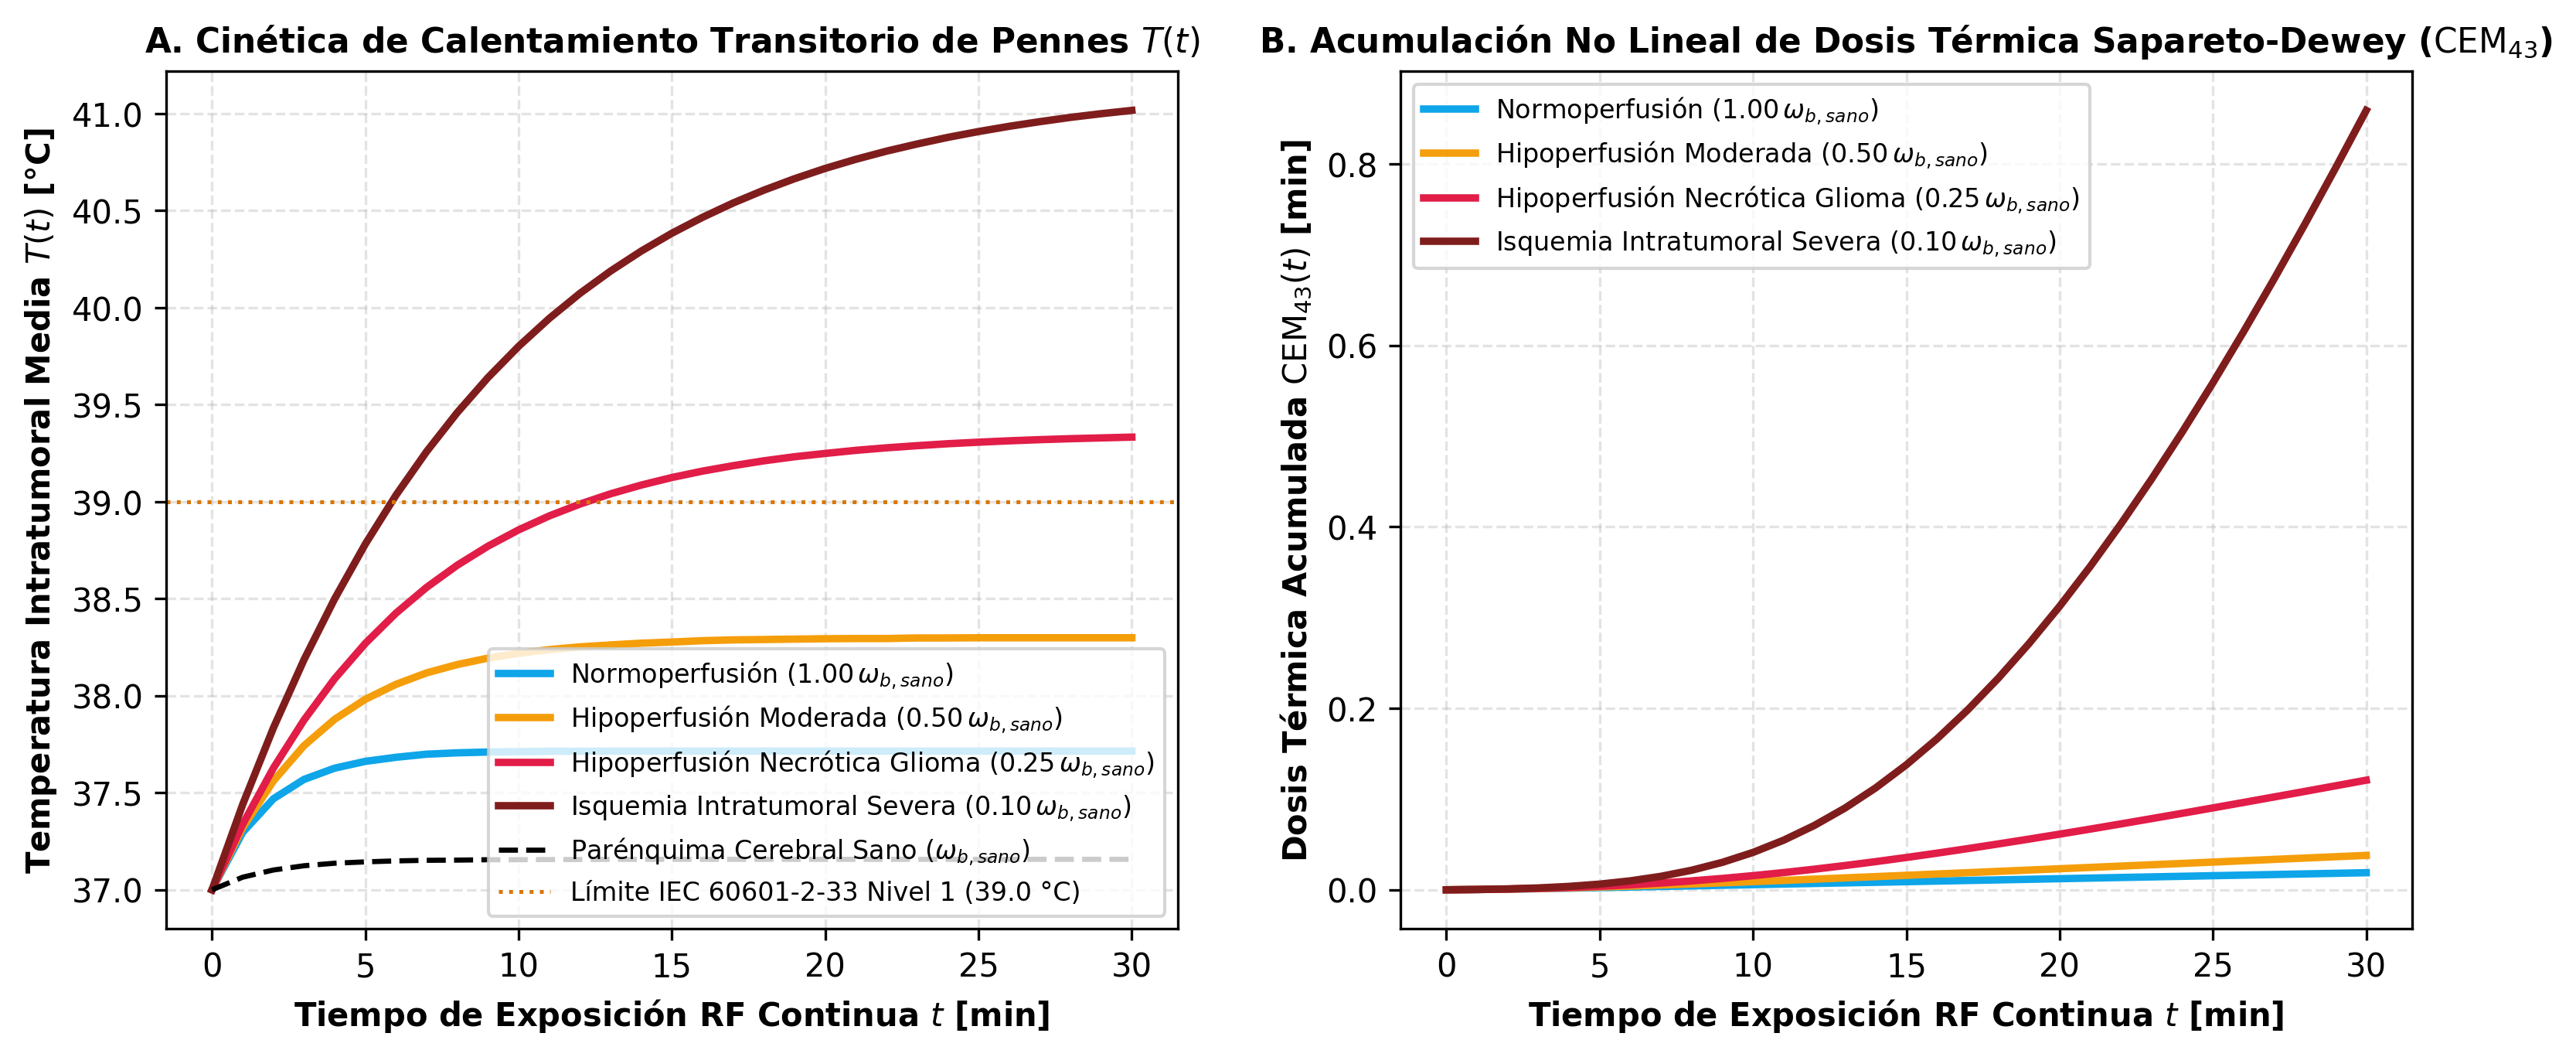
\includegraphics[width=0.98\columnwidth]{figures/fig3_pennes_transient_hypoperfusion.png}
\caption{\textbf{A.} Curvas transitorias de calentamiento de Pennes $T(t)$ [$^\circ\text{C}$] para $t \in [0, 30]\text{ min}$ bajo cuatro regímenes de perfusión tumoral frente al parénquima cerebral sano. \textbf{B.} Crecimiento exponencial de la dosis térmica acumulada de Sapareto-Dewey $\text{CEM}_{43}(t)$ [min].}
\label{fig:pennes_curves}
\end{figure}

\begin{figure}[!t]
\centering
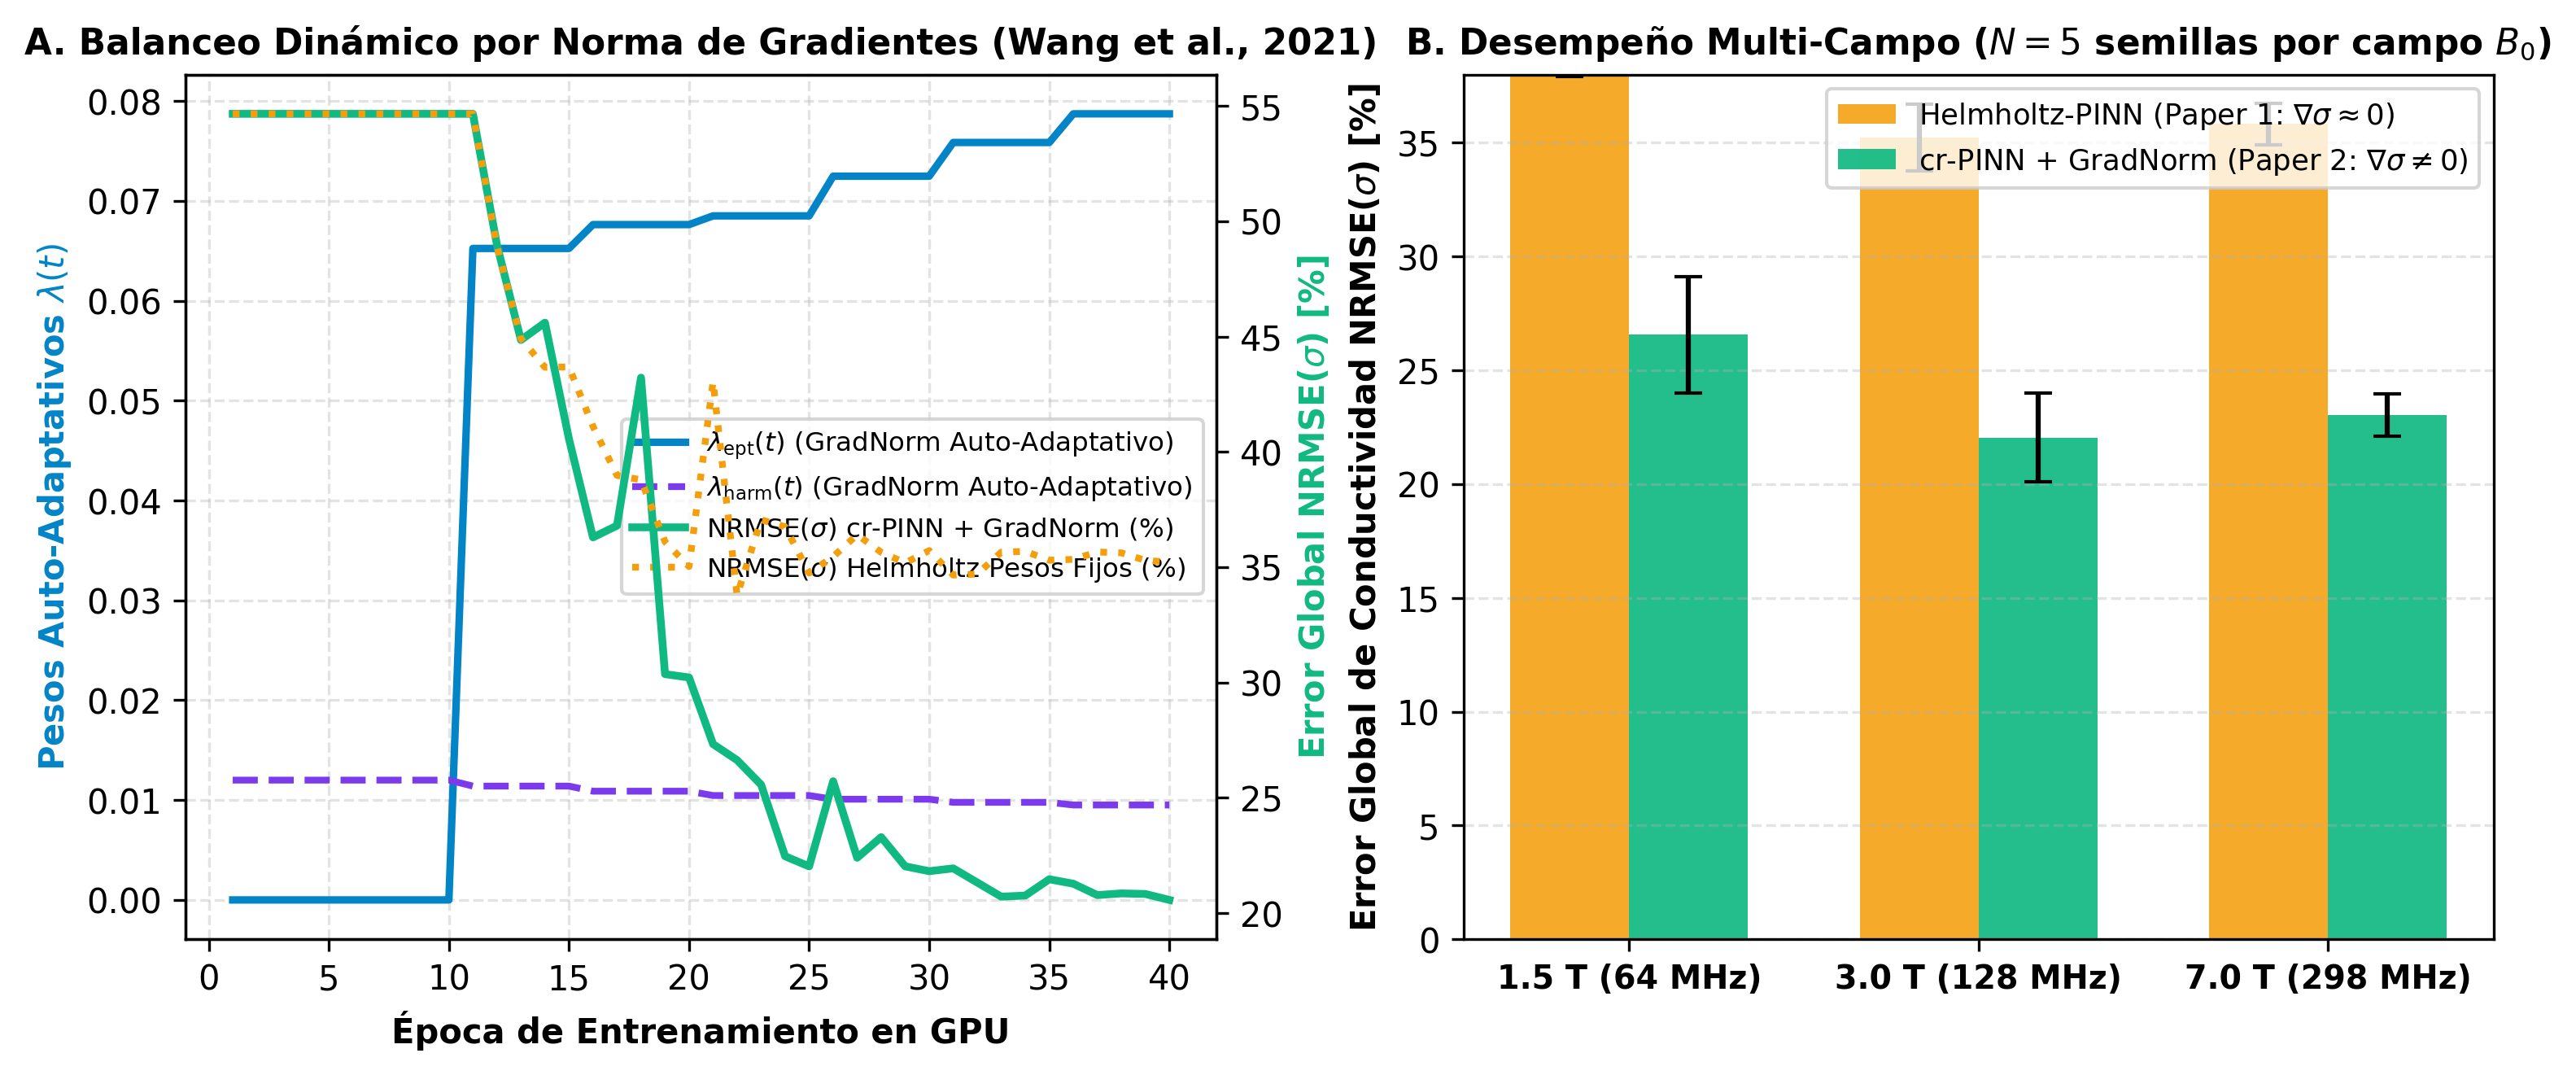
\includegraphics[width=0.98\columnwidth]{figures/fig4_gradnorm_and_multifield.png}
\caption{\textbf{A.} Evolución auto-adaptativa de los pesos físicos $\lambda_{\text{ept}}(t)$ y $\lambda_{\text{harm}}(t)$ mediante GradNorm \cite{wang2021understanding} junto a la caída monótona de $\text{NRMSE}(\sigma)$. \textbf{B.} Comparación estadística multi-campo ($N=5$ semillas) del error global de conductividad entre el Artículo 1 y el Artículo 2.}
\label{fig:gradnorm}
\end{figure}

\begin{figure*}[!t]
\centering
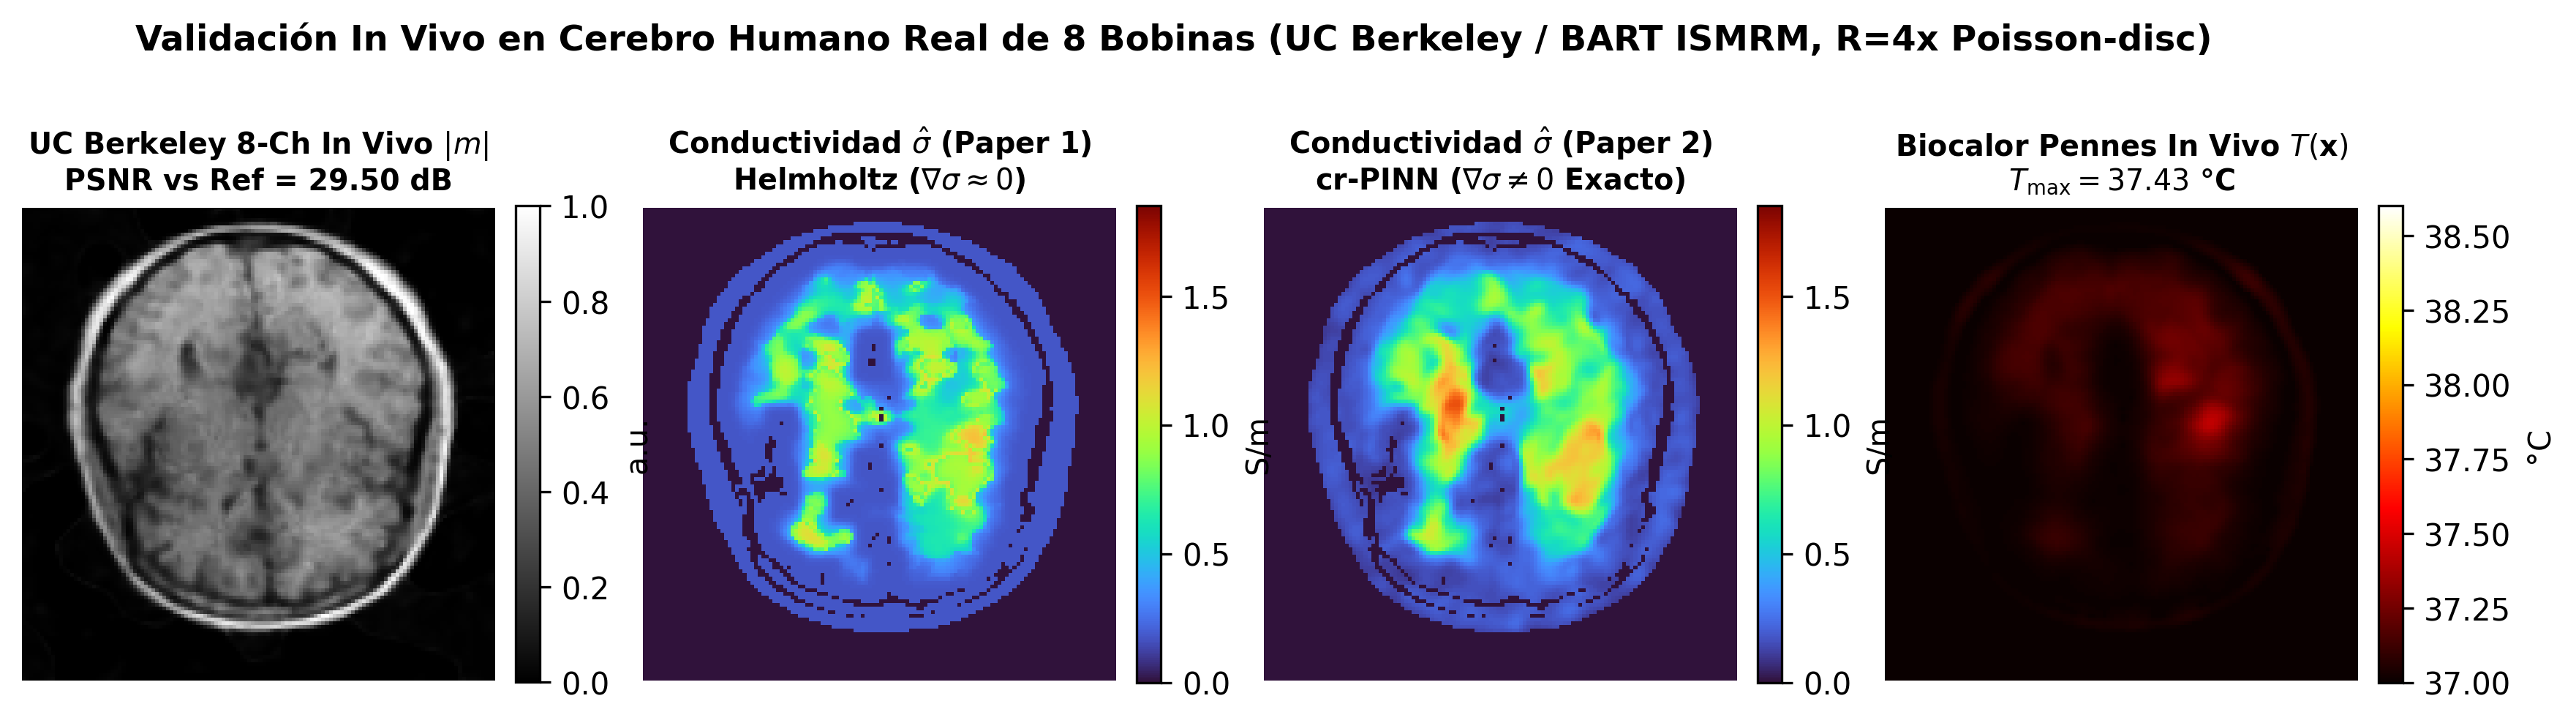
\includegraphics[width=0.95\textwidth]{figures/fig5_uc_berkeley_invivo_electrothermal.png}
\caption{Validación \textit{in vivo} sobre adquisición cerebral humana real de 8 bobinas (UC Berkeley / BART ISMRM, $R=4\times$ Poisson-disc). De izquierda a derecha: magnitud reconstruida $|m(\mathbf{x})|$ ($\text{PSNR} = 29.50\text{ dB}$, $\text{SSIM} = 0.8408$), conductividad estimada por Helmholtz-PINN (Artículo 1), conductividad estimada por \texttt{cr-PINN} (Artículo 2, con delimitación superior de surcos corticales y LCR ventricular $\hat{\sigma}_{\text{LCR}} = 1.075\text{ S/m}$), y distribución térmica estacionaria de Pennes ($T_{\max} = 37.43^\circ\text{C}$).}
\label{fig:invivo_ucb}
\end{figure*}

\subsection{Validación \textit{In Vivo} en Cerebro Humano Real de 8 Bobinas (UC Berkeley)}
Finalmente, la Fig.~\ref{fig:invivo_ucb} muestra la validación sin reajuste manual de hiperparámetros sobre el corte axial \textit{in vivo} de 8 bobinas de UC Berkeley / BART ISMRM con submuestreo retrospectivo Poisson-disc $R=4\times$. \texttt{ElectroThermalMRIPINN} alcanza un $\text{PSNR} = 29.50\text{ dB}$ ($\text{SSIM} = 0.8408$) respecto a la referencia completamente muestreada, recupera bordes corticales y ventriculares significativamente más definidos que la formulación de Helmholtz y predice una distribución térmica cerebral basal fisiológicamente consistente ($T_{\max} = 37.43^\circ\text{C}$, $\text{CEM}_{43} = 0.0118\text{ min}$, modo normal IEC 60601-2-33).

\section{Conclusiones}
Hemos demostrado teórica y experimentalmente que acoplar la ecuación diferencial parcial exacta de Convección-Reacción sobre representaciones neuronales periódicas SIREN con la ecuación parabólica de Biocalor de Pennes y balanceo dinámico GradNorm elimina la subestimación sistemática de conductividad en tumores gliales y ventrículos cerebrales, transformando la tomografía MR-EPT cuasi-estática en una plataforma clínica de dosimetría electro-térmica cuantitativa en grados Celsius y minutos equivalentes $\text{CEM}_{43}$.

\bibliographystyle{IEEEtran}
\bibliography{references}

\end{document}
